\documentclass[12pt, a4paper, openany]{report}

\usepackage{amsmath,amsfonts,amssymb}
\usepackage{graphicx}
\usepackage[colorlinks=true, allcolors=blue]{hyperref}
\usepackage{}


\begin{document}

\title{SMILE\\
SEM Image Lines Estimator}
\author{Iacopo Mochi}
\date{\today}

\maketitle


\chapter{SMILE image analysis in three steps}
SMILE can  be run as a standalone application for macOS or Windows, or as MATLAB application running \textbf{SMILE.mlapp} from the MATLAB App Designer.
\section{Step 1: Loading the images}
\begin{figure}[hbtp]
	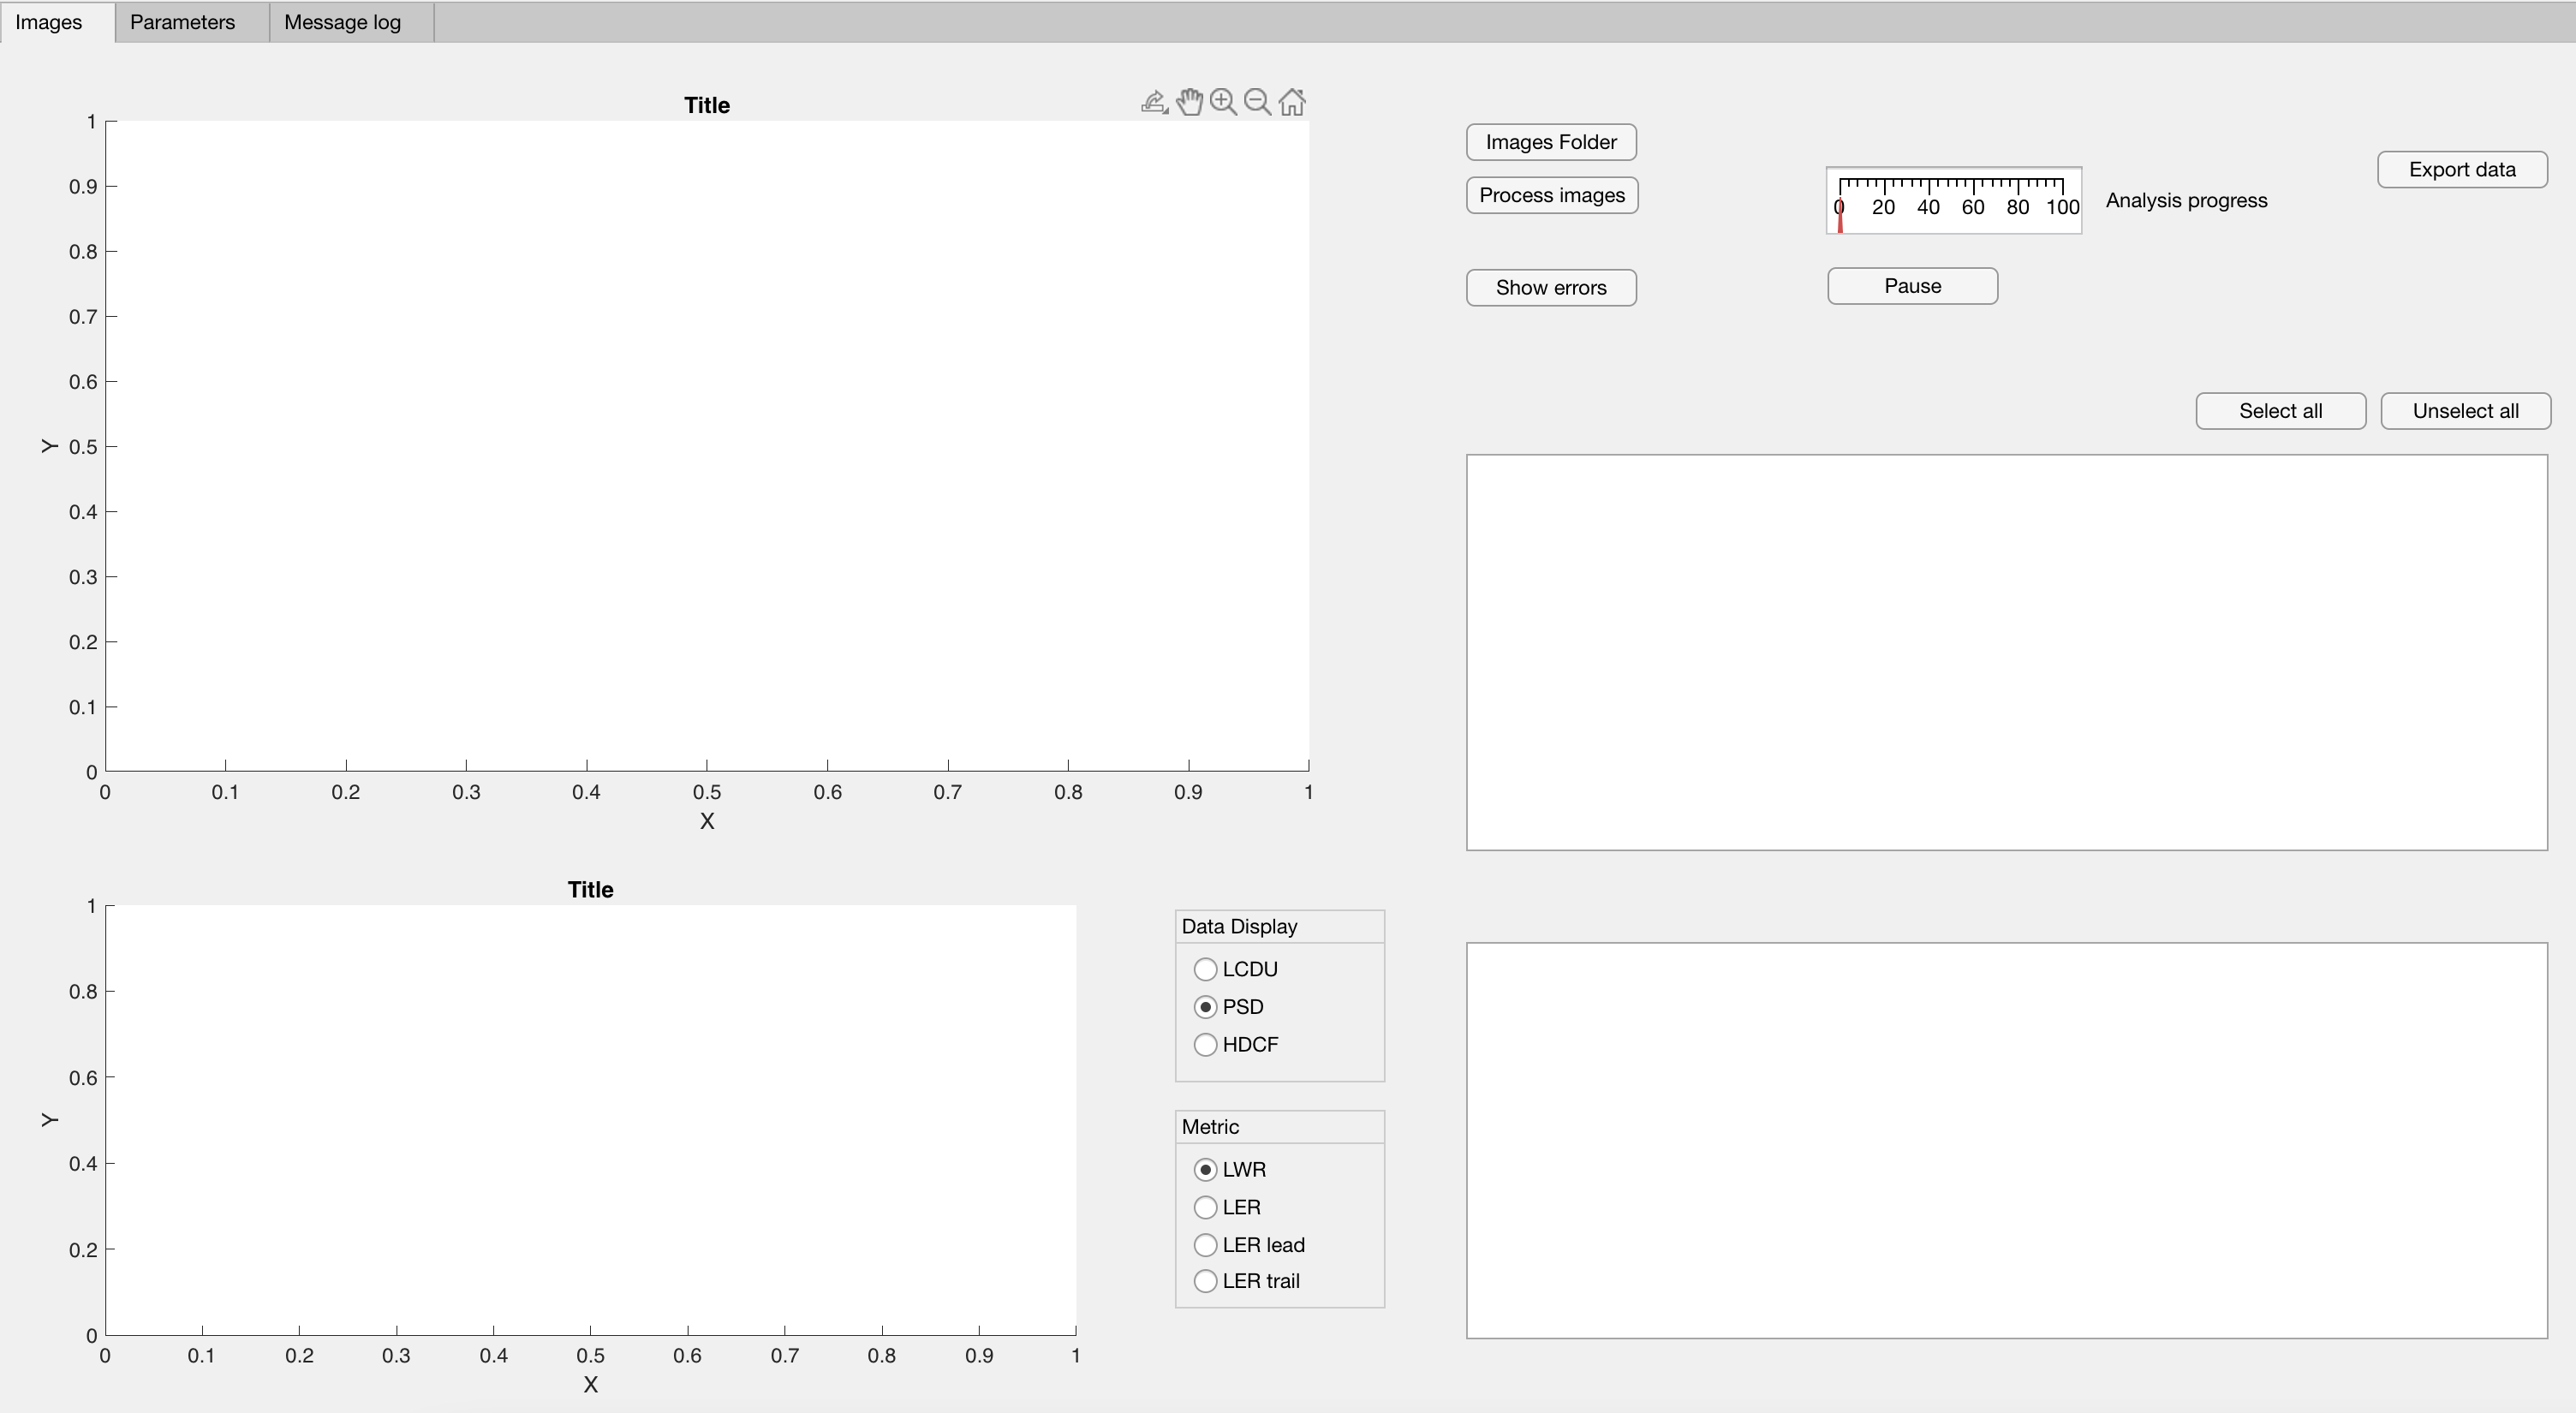
\includegraphics[width=\textwidth]{figures/GUI_01.png}
	\caption{SMILE user interface: ``\emph{Images}" tab.}
	\label{fig:GUI_01}
\end{figure}
The first step is to click on the \textbf{Images Folder} button and select the folder containing the SEM images to analyze. The images must be in TIF or JPG format. The program will try to load all the images in the folder and it will display the first unprocessed image in the top left box. The units displayed are pixels. The tables on the right will be populated with a list of the file names. By selecting a different row in the table, the corresponding image will be visualized. See figure \ref{fig:GUI_01}. SMILE relies on a pre-trained neural network to distinguish images with Line/Space and Contacts arrays. The top table will be populated with the former and the bottom one with the latter. It is also possible to turn off the automatic image classification by toggling the button \textbf{Automatic feature recognition} in the \emph{images} panel (Figure \ref{fig:GUI_01A}). In this case, when the \textbf{Images Folder} button is pressed, all the images are loaded as lines and spaces. The user can select each row and move images with contact arrays to the bottom table by pressing the ``t'' key. 

In general, to change the image type from contacts to lines and vice versa, it is sufficient to select the relative row in the data table and press the ``t'' key.
\begin{figure}[hbtp]
	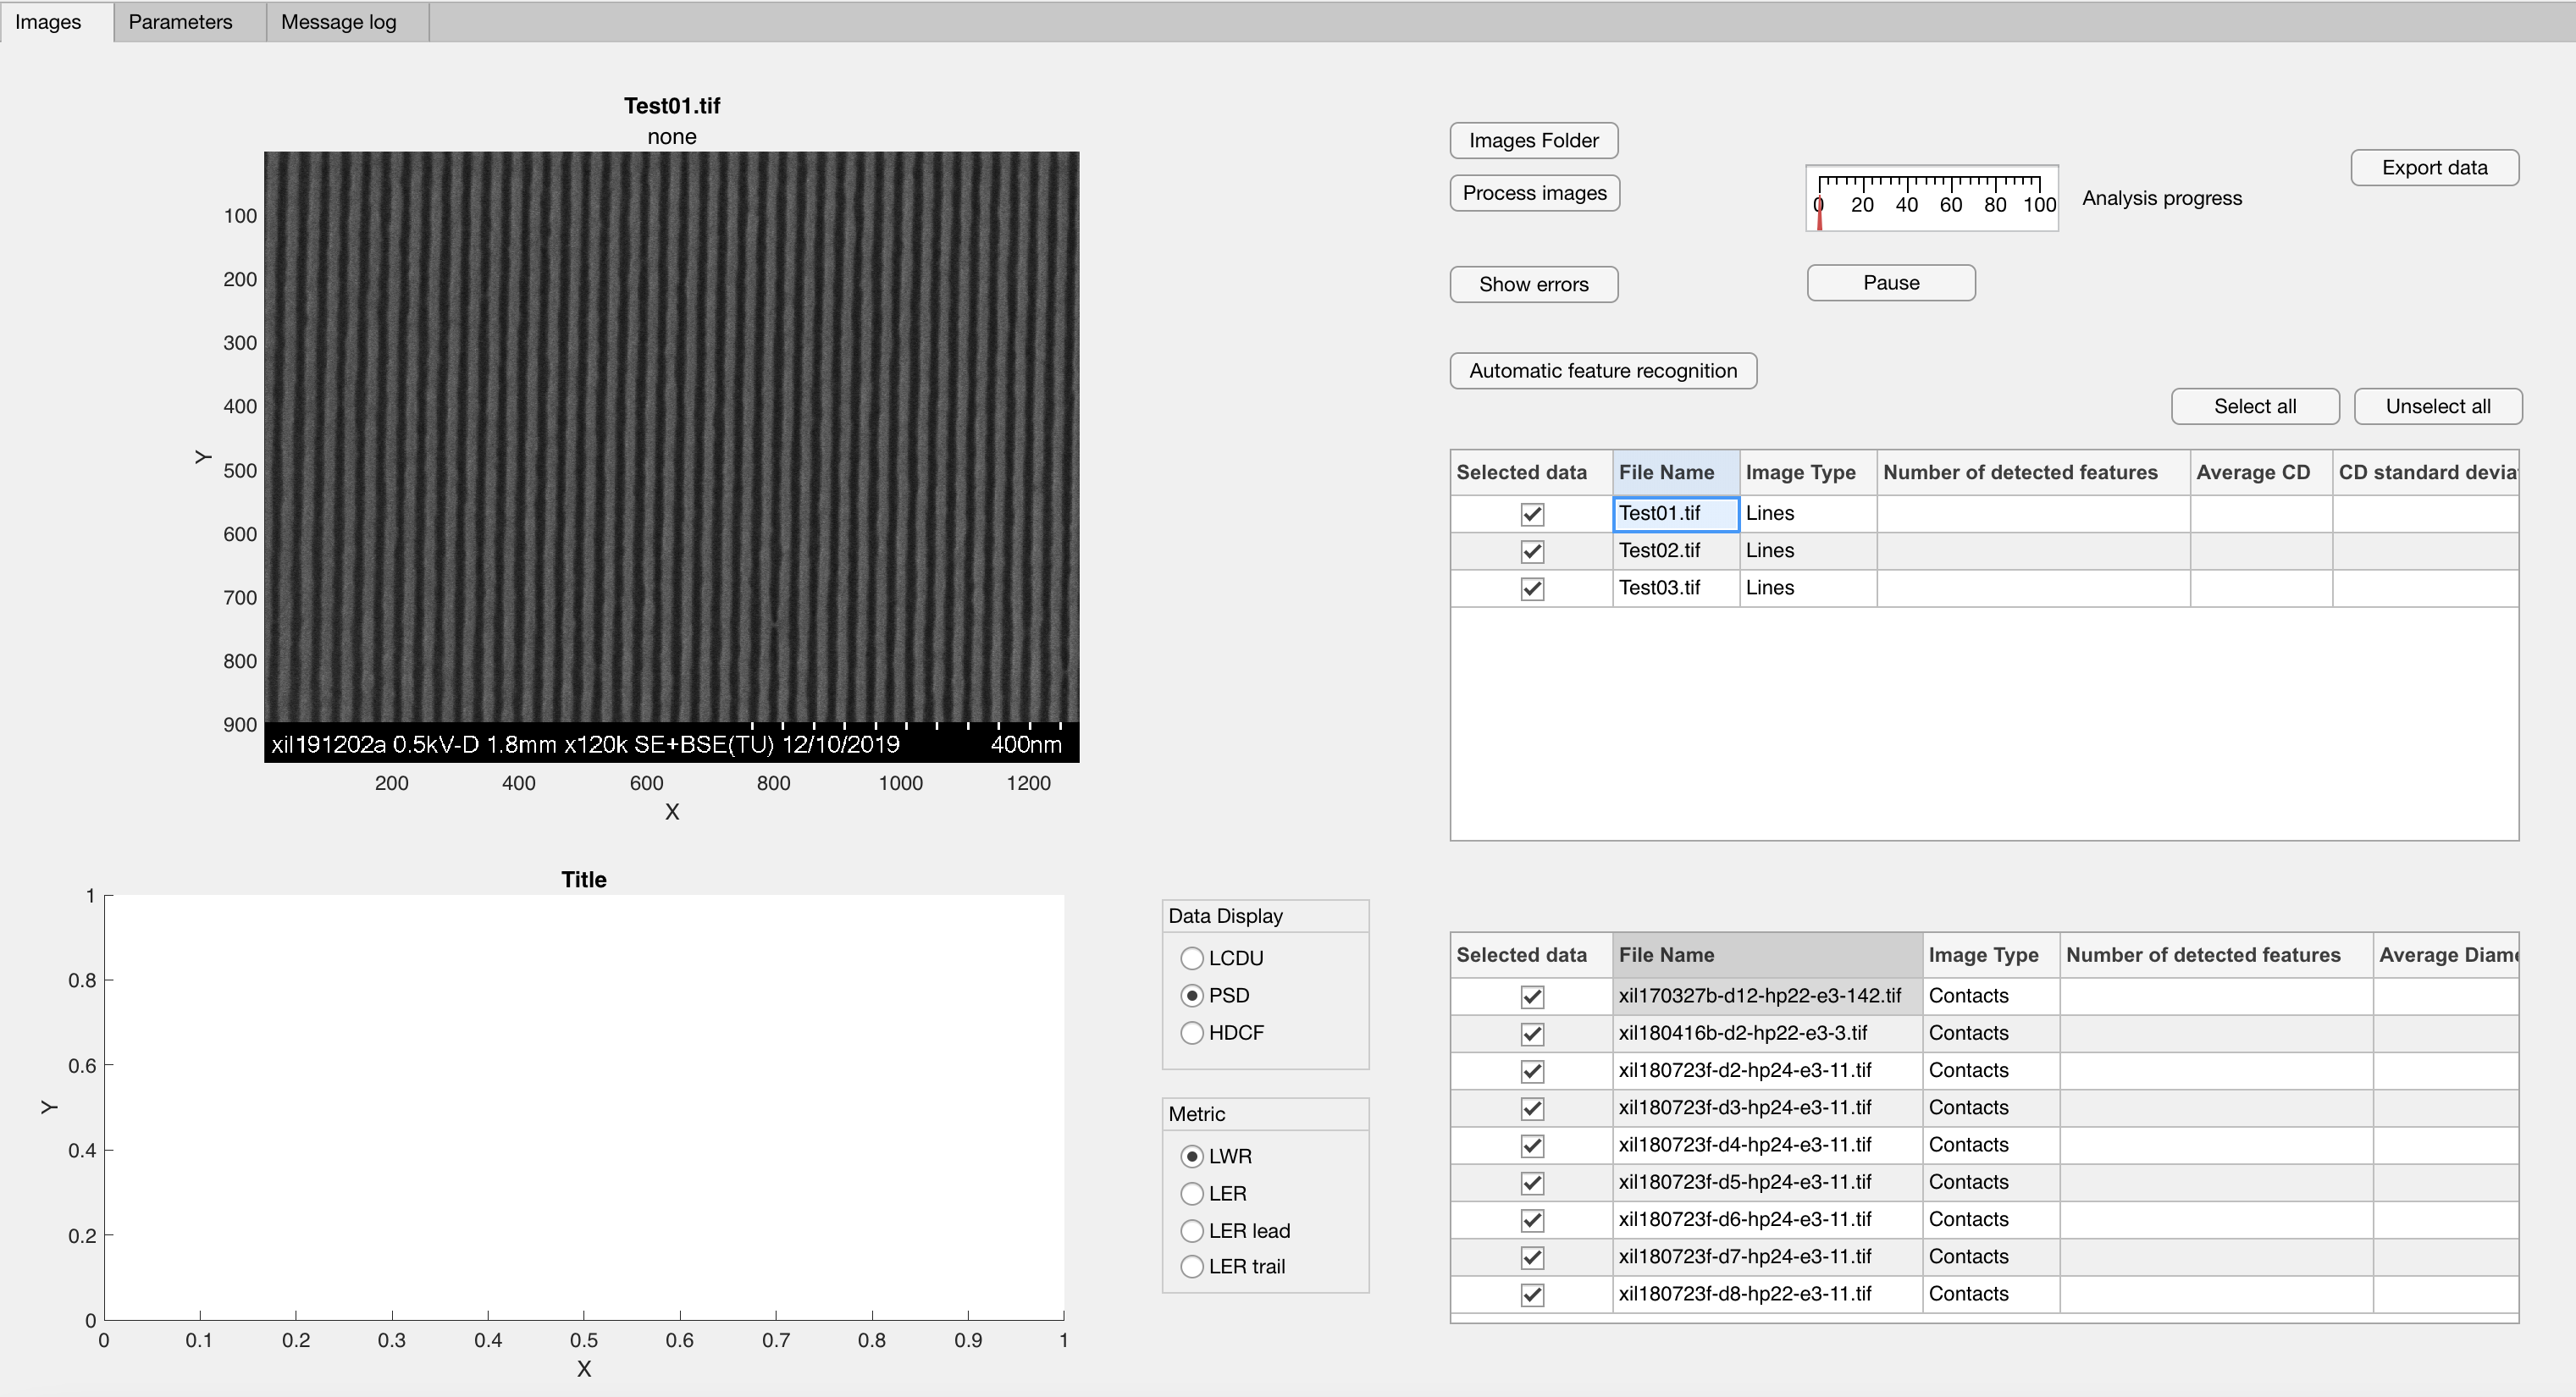
\includegraphics[width=\textwidth]{figures/GUI_01A.png}
	\caption{SMILE user interface: ``\emph{Images}" tab. After selecting the image folder, SMILE will populate the tables and display the first unprocessed image.}
	\label{fig:GUI_01A}
\end{figure}
\section{Step 2: Setting the parameters}
The second step is setting the parameters for the analysis. This is done in the ``\emph{Parameters}" tab as shown in figure \ref{fig:GUI_02A}. The parameters can be set manually, or imported from a predefined parameter file using the \textbf{Load parameters} button. Usually, the first parameter to set is the region of interest. This is done by clicking the \textbf{Set ROI} button and dragging a rectangle on the image displayed over the area that needs to be analyzed (Figure \label{fig:GUI_02A}). Another important parameter to set is the pixel size. The pixel size can be retrieved automatically for images collected at PSI. To do this, the SEM model drop down menu should be set to ``Hitachi'' or ``Zeiss'', depending on the model used. If the SEM model is set to ``Generic'', the software will read the value (expressed in  nanometers) in the \textbf{Pixel size} text box.
\begin{figure}[thbp]
	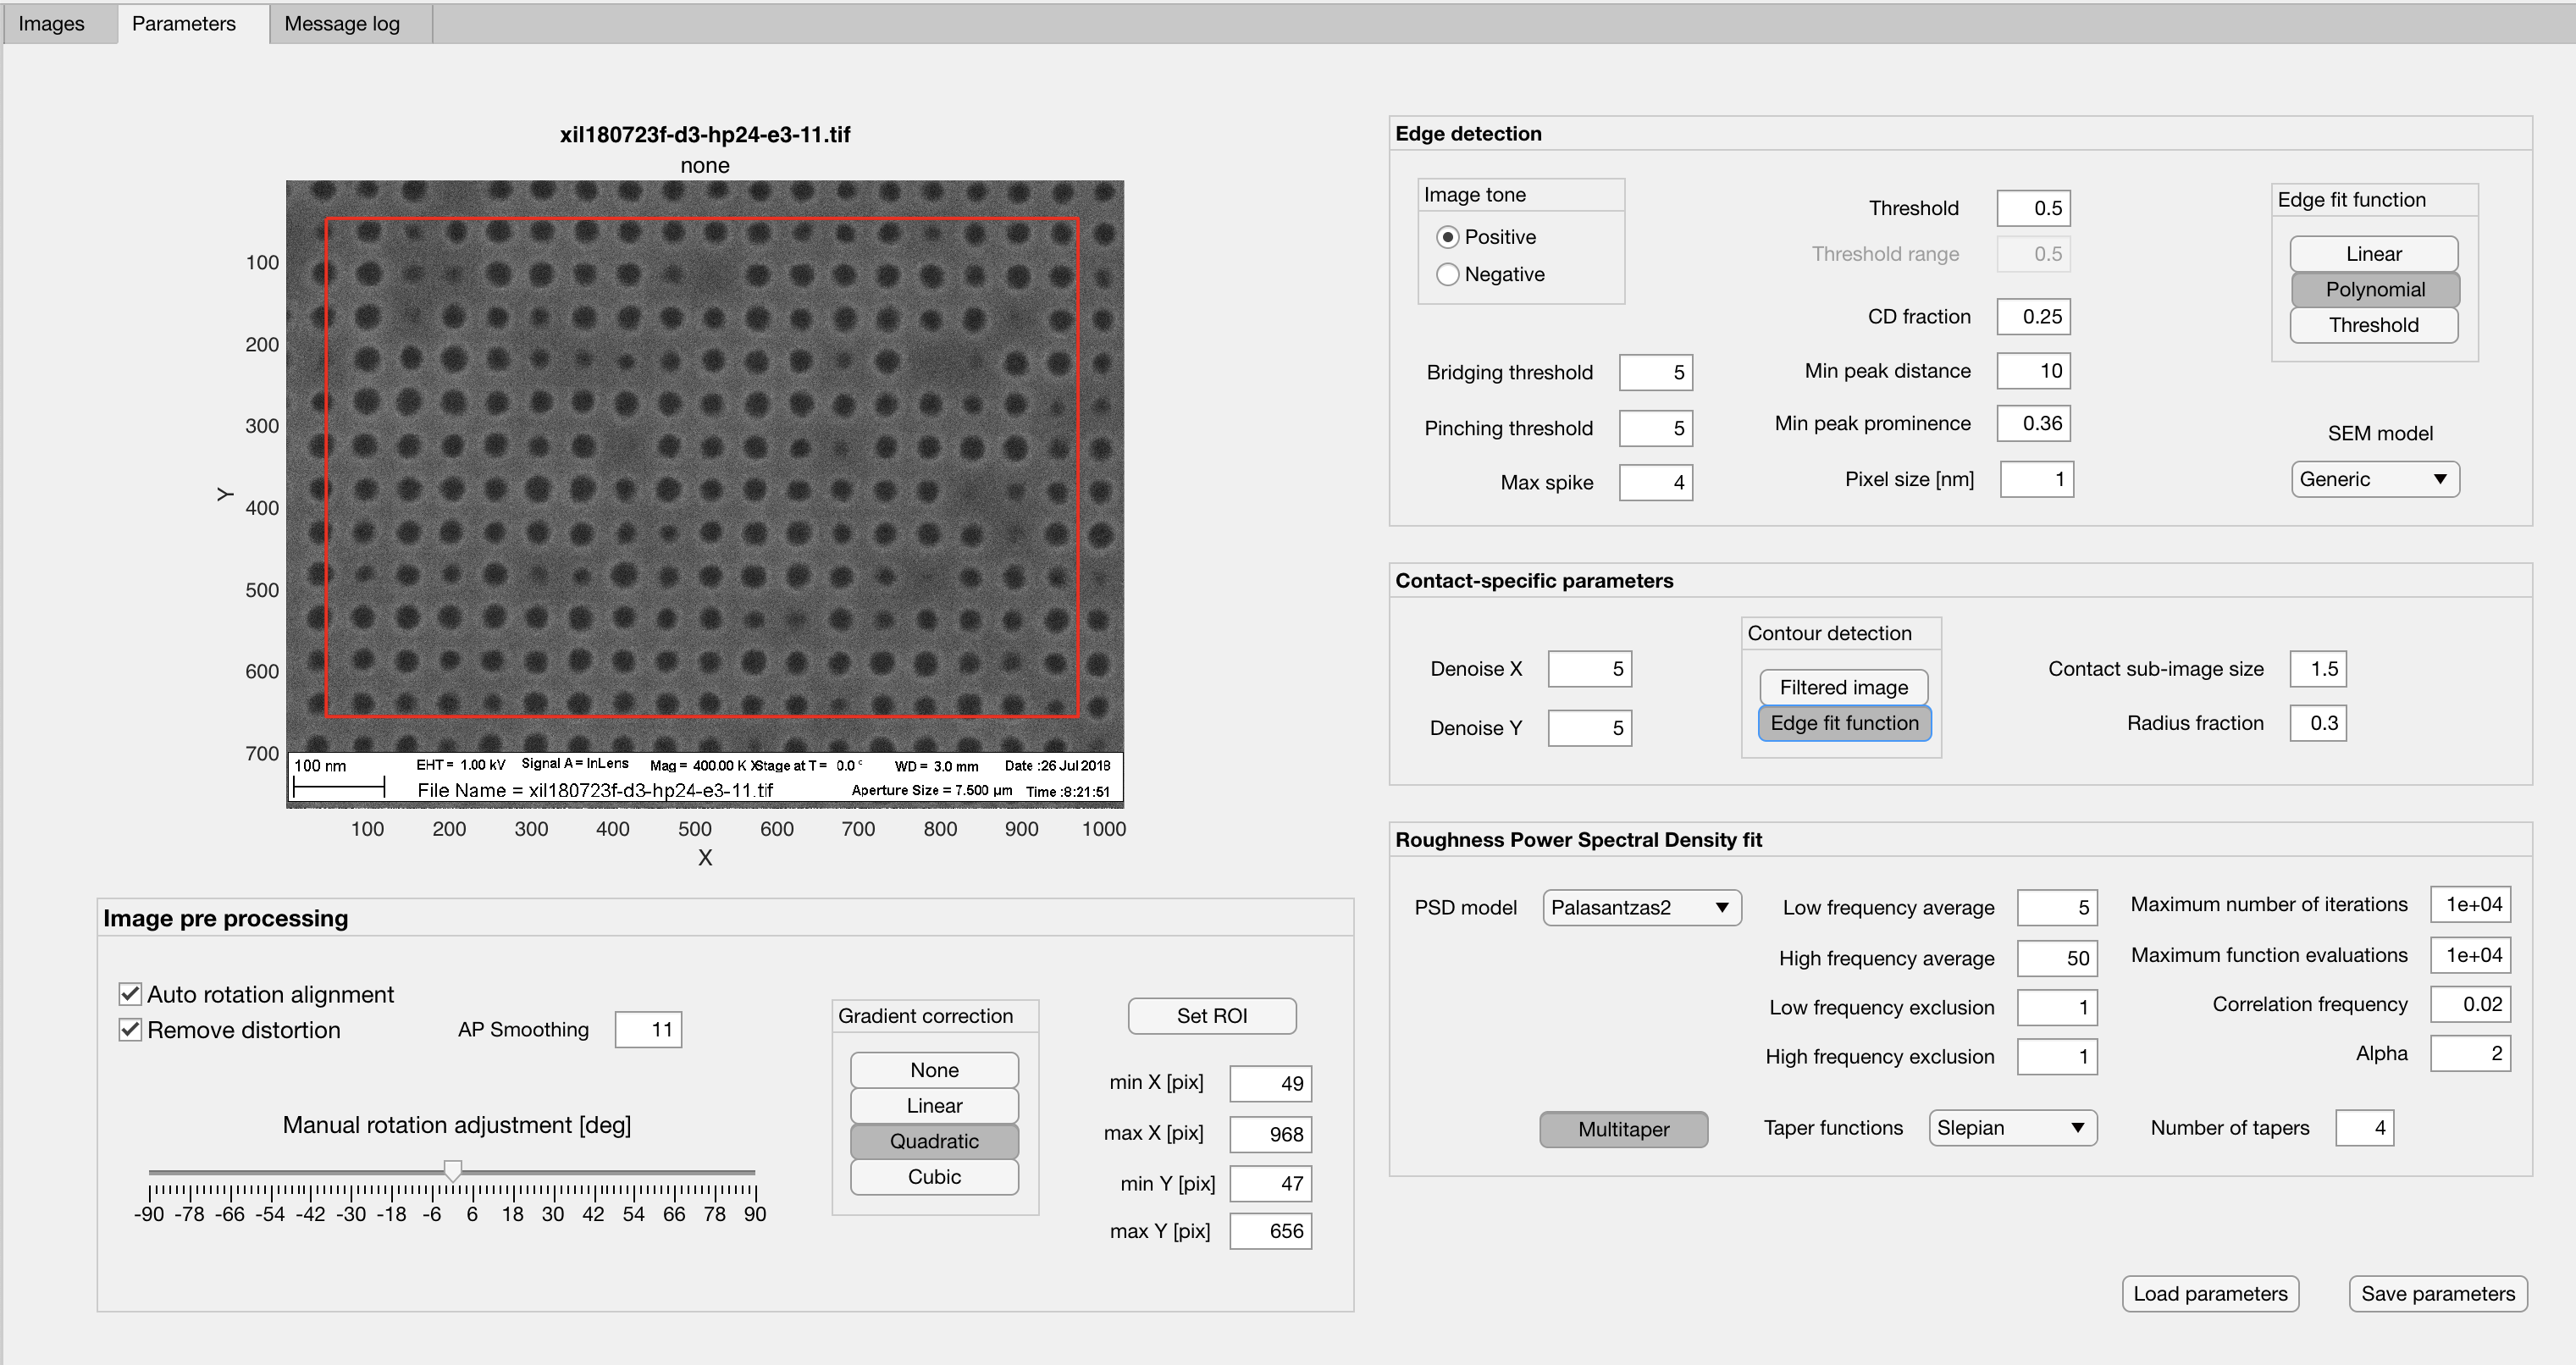
\includegraphics[width=\textwidth]{figures/GUI_02A.png}
	\caption{SMILE user interface: ``\emph{Parameters}" tab.}
	\label{fig:GUI_02A}
\end{figure}
\section{Step 3: Run the analysis}
The third step is the image analysis which is performed from the ``\emph{Images}" tab pressing the \textbf{Process images} button. As the images are analyzed, the software fills the data table with the measured values and displays the detected contours of the image features as shown in figure \ref{fig:GUI_01B}.
\begin{figure}[htbp]
	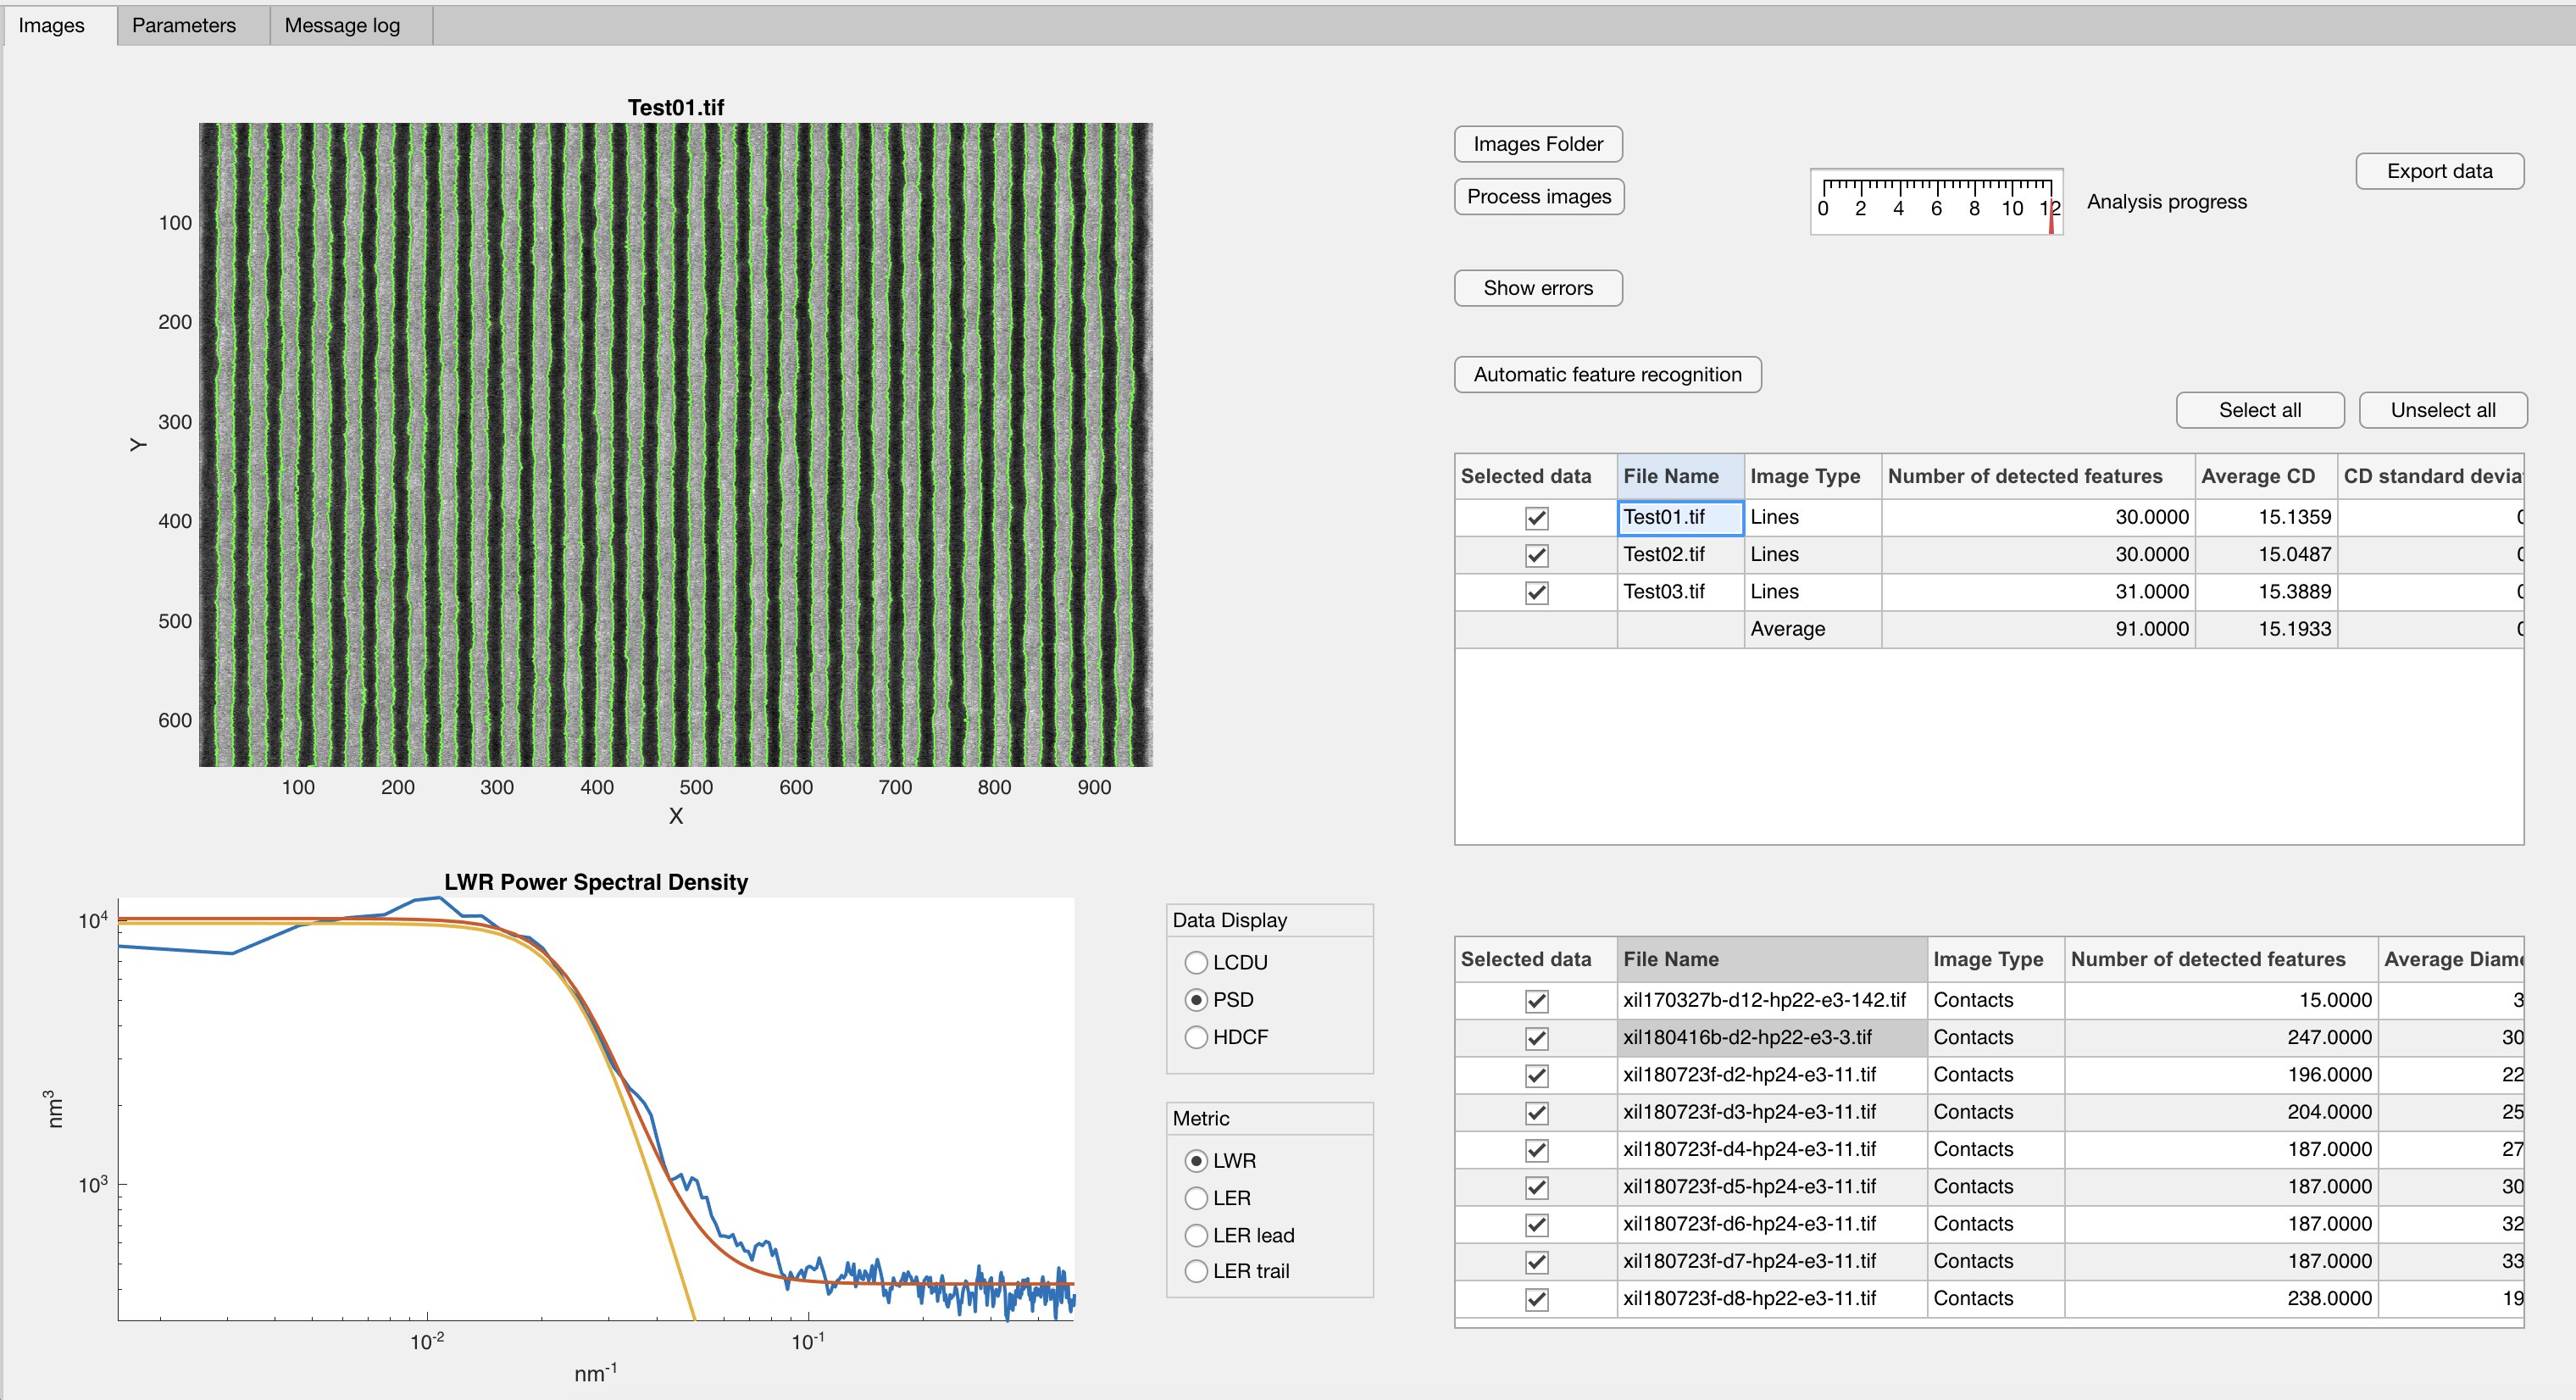
\includegraphics[width=\textwidth]{figures/GUI_01B.png}
	\caption{SMILE user interface: ``\emph{Images}" tab. After processing the images the detected contours of the image features are overlayed to the original image. Press the \textbf{Show Errors/Hide Errors} button to display or hide edge detection failures or bridging/pinching defects.}
	\label{fig:GUI_01B}
\end{figure}
%\chapter{Parameters}
%The image processing parameters are accessible from the ``\emph{Parameters}" tab. Once the parameters are set, they can be saved using the button \textbf{Save parameters} and reloaded using the button \textbf{Load parameters}. The software stores all the parameters with the exception of the SEM model and the PSD model. Note that every SEM will have, in principle, a different set of parameters which should be inter-calibrated to compare the measured CD and LWR values.
%\section{Edge detection parameters}
%\subsection{Region of interest -- ROI}
%Click the ROI button to set the region of interest where the analysis is going to be performed. Then drag a rectangle over the image on the left corresponding to the desired ROI. 
%\begin{figure}[hbt]
%	\includegraphics[width=\textwidth]{figures/select_ROI.png}
%	\caption{SMILE user interface: ROI selection.}
%	\label{fig:select_ROI}
%\end{figure}
%\subsection{Threshold}
%The edge of the lines is detected at a specific threshold relative to the normalized intensity of the image ROI. The threshold value in nanometers is specified in the Threshold text box and, in principle, it depends on the SEM settings. An ideal calibration experiment would be performed collecting an image of a line/space pattern with a known CD using a specific set of SEM parameters and a specific microscope. The threshold value would then be adjusted to match the expected CD value.
%\subsection{Maximum spike}
%With noisy SEM images, there is always a chance that a stray noise peak tricks the edge detection algorithm into creating an artificial spike in the line profile. The Maximum spike value is the maximum allowed value in the edge derivative. Any point in the detected profiles for which the local derivative exceeds the value specified in the text box is substituted with the profile average value for the LWR analysis. The choice of the value of this parameter can be made by observing the profiles and estimating the impact of noise by eye. Values below 4 are not recommended as the filter would likely smooth the real edge profiles.
%\subsection{CD Fraction}
%The edge detection algorithm looks for the edges of the line using data included in an interval of the line intensity profile centered on the average profile positions. The size of this interval is defined by the CD fraction value. Recommended values are between 0.1 and 0.45 depending on the selected edge detection algorithm.
%\subsection{Minimum peak distance}
%This parameter is the minimum distance in pixels between the profiles. Setting this parameter allows to exclude spurious edges that might be detected in the presence of lines with pronounced trapezoidal topography. The general rule for this parameter is to keep it just larger than the smallest distance expected between the edges.
%\subsection{Minimum peak prominence}
%As the minimum peak distance, the minimum peak prominence is a parameter used to help the edge detection algorithm to find the correct profiles. The default value is 0.36. if you notice any missing profile after processing the image, you can increase the value, if you see more profiles than expected, you can reduce it. 
%\subsection{Auto alignment}
%The software is designed to detect vertical line profiles. Sometimes, SEM images are not perfectly aligned; check this box to correct the alignment of the image if necessary, but be advised that this procedure may alter the spectral content od the profiles. In the current version of SMILE the image rotation algorithm uses a nearest-neighbour interpolation.
%\subsection{Remove distortion}
%When you check this box, the software removes any average distortion in the lines profiles induced by the SEM. When the microscope operates in line-scan mode, a thermal or mechanical drift of the stage can induce some line bending for example.
%\section{LWR calculation parameters}
%The LWR is calculated from the integral of the power spectral density (PSD). The program calculates the average PSD of the line width and tries to fit it to a model in order to estimate the correlation frequency and the bias. The following parameters are used to give the software first guess for the fitting procedure.
%\subsection{PSD model}
%The available models for the PSD fit are:
%\begin{itemize}
%\item Gaussian
%\item FloatingAlpha
%\item NoWhiteNoise
%\item Palasantzas1
%\item Palasantzas2
%\item Integral
%\end{itemize}
%The Palasantzas2 \cite{PhysRevB.48.14472} model is a commonly used standard and it is the recommended value for this parameter. The model is described by:
%\begin{equation}
%    PSD(\nu)=\frac{\xi\sigma^2}{\left(1+a\xi^2 \nu^2\right)^{1+\alpha}}+Nl
%    \label{eq:palasantzas}
%\end{equation}
%where $\xi$ is the correlation length and $\alpha$ is the roughness exponent, or Hurst coefficient and Nl is the high-frequency noise background. More information on the implementation of this and other PSD models can be found in a paper published in the proceedings of the SPIE Photomask Technology conference 2020.\cite{Mochi_SMILE}
%\begin{figure}[hbt]
%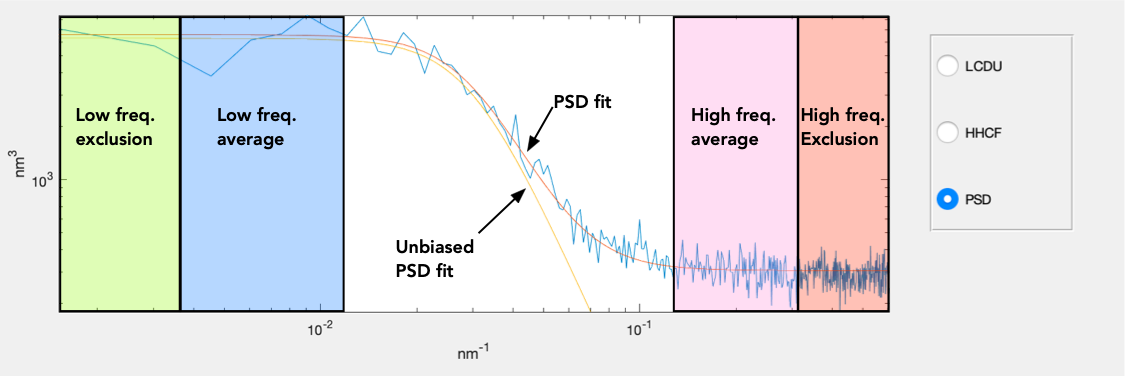
\includegraphics[width=\textwidth]{figures/PSD_01.png}
%\caption{PSD curve plot and fit.}
%\label{fig:PSD01}
%\end{figure}
%\begin{figure}[hbt]
%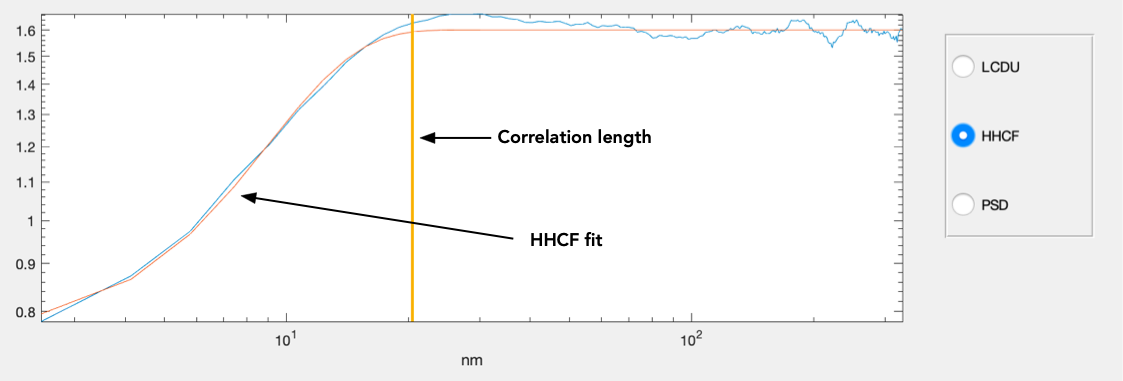
\includegraphics[width=\textwidth]{figures/HHCF_01.png}
%\caption{Height-height correlation function curve plot and fit. The vertical yellow line shows the estimated value of the correlation length.}
%\label{fig:HHCF01}
%\end{figure}
%\subsection{Low frequency average}
%After processing the images, the PDS curve is displayed in the ``\emph{Lines}" tab. The low frequency average value is the number of frequency values averaged to determine a first guess of the parameter $\sigma$ in equation \ref{eq:palasantzas}. Recommended values range from 5 to 10.
%\subsection{High frequency average}
%The high frequency average value is the number of frequency values averaged to determine a first guess of the parameter $Nl$ in equation \ref{eq:palasantzas}. Recommended values range from 50 to 100.
%\subsection{Low frequency exclusion}
%This parameter gives the chance to exclude the first frequency components from the estimate of the low frequency average and from the PSD fit. The minimum recommended value for this parameter is currently 1.
%\subsection{High frequency exclusion}
%This parameter gives the chance to exclude the last frequency components from the estimate of the high frequency average  and from the PSD fit. The minimum recommended value for this parameter is currently 0.
%\subsection{Maximum iterations/function evaluations}
%These two parameters are relevant for the behaviour of the fitting algorithm. It is recommended to keep their values to the default 10000. If the value of on e of the two parameters is set too low, a warning message will be displayed on the MATLAB command window while the images are being processed.
%\subsection{Correlation frequency}
%The correlation frequency corresponds to the point where the PSD curve bends downward as shown in figure \ref{fig:PSD01}. The value is expressed in nm$^{-1}$. The recommended value is 0.02, but a better estimate can be made in each case looking at the PSD curve or at the correlation length shown in the HHCF plot (see figure \ref{fig:HHCF01}).
%\subsection{Alpha}
%This is the the $\alpha$ coefficient in equation \ref{eq:palasantzas}. Recommended values go from 0.2 to 2.
%\subsection{SEM model}
%The SEM model parameter can be set as Hitachi, Zeiss and Manual. \textbf{For usage with images not collected at PSI, it is necessary to use the Manual setting}. For images collected at PSI, if the SEM model is known, setting this parameter will allow the code to read in the pixel size value from the images and override the Pixel size parameter.
\bibliography{bibliography}
\bibliographystyle{ieeetr}
\end{document}